\subsection{Yang--Mills and Hodge: crossing on the open steps}\label{ssec:headline}

The crossing network of the package (Section~\ref{ssec:crossing} describes it on a calibration problem) is aimed here at the open leaves of the two trees. Every construction of its library is a typed node: it gives an output of one type and needs inputs of others. The Yang--Mills library holds the single-link law of $\mathrm{SU}(2)$, which is a von Mises--Fisher law on $S^{3}$; the sharp quarter inequality $W_{1}(\nu_{b},\nu_{b'})\le\frac14|b-b'|$ of \cite{BB26d}; Dobrushin's uniqueness criterion \cite{Dob68}; three dependency graphs of the links (no gauge fixing, temporal gauge, and the maximal-tree gauge of Creutz \cite{Cre77} with one fixed link in every plaquette); reflection positivity and the transfer matrix \cite{OSei78}; the gauge Dobrushin--Shlosman criterion and the Bakry--\'Emery bound of \cite{SZZ23}; the Polchinski flow and the multiscale log-Sobolev inequality \cite{BB21}; Ba{\l}aban's renormalisation group \cite{Bal87}; and a finite subgroup of $\mathrm{SU}(2)$. The Hodge library holds Markman's theorem on Weil classes of abelian fourfolds \cite{Mar25w}, the reduction of Moonen and Zarhin in dimension at most five \cite{MZ98}, Schoen's products \cite{Sch98p}, Shioda's structure of Fermat varieties \cite{Shi79}, the Hodge characters of the Fermat fourfold of degree $110$ left by the census of \cite{BB26c}, Buskin's theorem on Hodge isometries of K3 surfaces \cite{Bus19}, and an unrefereed claim of the Hodge conjecture for CM abelian varieties \cite{OAI26b}. Two nodes cross when the output of one is an input of the other. An offspring that needs nothing more is closed and goes to its check, a computation that accepts, rejects with the measurement that stopped it, or stops when no checkable form exists. Checked offspring join the pool and seed the next generation.

\begin{figure*}[t]
\centering
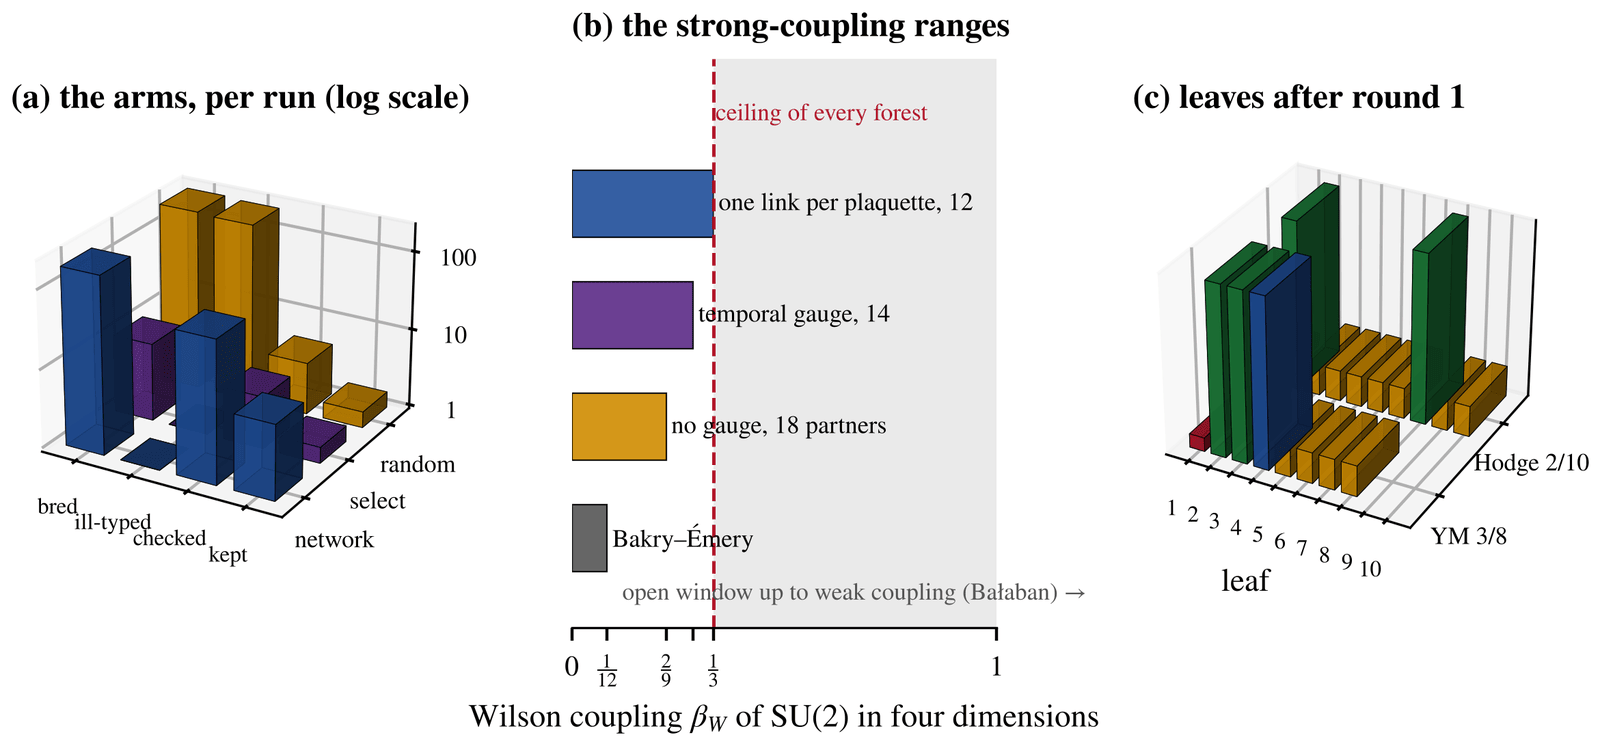
\includegraphics[width=0.98\textwidth]{figures/fig_headline}
\caption{The first headline round. (a) Offspring bred, ill-typed, checked and kept per run of each arm, on a logarithmic scale. The network enumerates the typed crosses; select draws pairs at random and keeps those whose types fit; random crosses whatever the types. (b) The ranges of four-dimensional $\mathrm{SU}(2)$ on which a lattice mass gap is proved: Bakry--\'Emery \cite{SZZ23}, single-link Dobrushin without gauge fixing \cite{BB26d}, and after the temporal and the one-per-plaquette gauge fixings (Theorem~\ref{thm:onethird}). The dashed line is the ceiling of every forest gauge fixing (Proposition~\ref{prop:forestceiling}); beyond it the window up to weak coupling is open. (c) The leaves of the two trees after the round, in the order of Table~\ref{tab:closure}: proved (green, the new step in blue), open (amber) and blocked (red).}
\label{fig:headline}
\end{figure*}

\emph{The first round.} Over five seeds of five generations of $40$ crosses, the network bred $180$ offspring per run, checked $64$ and accepted $8$; select bred $8.8$, checked $3.6$ and accepted $0.6$; random bred $200$, of which $191.2$ were ill-typed, and accepted $0.6$ (Fig.~\ref{fig:headline}a). Every run of the network reached the composite of Dobrushin's criterion, the sharp quarter, the von Mises--Fisher law and the maximal-tree gauge, whose check counts $12$ active partners for every active link and accepts the range $\beta_{W}<\frac13$; no run of the controls reached it. The network enumerates every typed pair, so its runs do not depend on the seed. The composite was first proposed by the language-model proposer of the package, which suggested fixing a gauge to cut the number of partners; a satisfiability search found the pattern of Lemma~\ref{lem:forest}, Lean~4 checked its finite part, and the cross was then entered in the library, from which the network rederives it. The network therefore reproduces this step; it did not originate it.

\emph{The step.} We use the normalisation of \cite{SZZ23,BB26d}: the Wilson measure of $\mathrm{SU}(2)$ on a finite set of links has density $\exp(2\beta\sum_{p}\mathrm{Re}\,\mathrm{Tr}\,U_{p})$ with respect to Haar measure, where $U_{p}$ is the ordered product around the plaquette $p$, and $\beta_{W}=4\beta$ is the coupling of the physics literature. A link of $\mathbb{Z}^{4}$ is written $(x,\mu)$ for the pair $\{x,x+e_{\mu}\}$; the plaquette at $x$ in the plane $\mu<\nu$ consists of the links $(x,\mu)$, $(x+e_{\mu},\nu)$, $(x+e_{\nu},\mu)$, $(x,\nu)$.

\begin{lemma}\label{lem:forest}
Let $\sigma\colon(\mathbb{Z}/2)^{4}\to\{0,1,2,3\}$ take the values $0,0,2,3,3,1,2,1,1,2,1,3,3,2,0,0$ at $x_{0}+2x_{1}+4x_{2}+8x_{3}=0,1,\dots,15$, and let $F$ be the set of links $(x,\sigma(x\bmod2))$, $x\in\mathbb{Z}^{4}$. Then
\begin{enumerate}[label=\textup{(\roman*)},leftmargin=*,itemsep=0pt]
\item every plaquette of $\mathbb{Z}^{4}$ contains exactly one link of $F$;
\item $F$ is a forest, and so is $F\cap E(\Lambda)$ for every set $\Lambda$ of sites, $E(\Lambda)$ being the links with both ends in $\Lambda$;
\item every link $e\notin F$ shares a plaquette with exactly $12$ links not in $F$, two in each of its six plaquettes.
\end{enumerate}
\end{lemma}

\begin{proof}
(i) The plaquette at $x$ in the plane $\mu<\nu$ contains $\#\{\sigma(x)\in\{\mu,\nu\}\}+[\sigma(x+e_{\mu})=\nu]+[\sigma(x+e_{\nu})=\mu]$ links of $F$, a number that depends only on $x\bmod2$ and the plane; inspection of the $16\times6=96$ cases of the table gives $1$ in each.\footnote{The inspection is a finite check. The eBLLM package carries it out in Lean~4, in the theorem \lean{one\_fixed\_per\_plaquette} of its file \lean{EBLLM/GaugeFix.lean}, proved by \lean{decide}, and repeated independently on a box of side six by \lean{verify\_gauge.py}. The table was found by a satisfiability search over the $4^{16}$ functions $\sigma$; it has eight solutions of period two, and none of period three.} (ii) Every site $x$ has exactly one link of $F$ leaving it in the positive direction, the link to $x+e_{\sigma(x)}$, and that link raises $h(x)=x_{0}+x_{1}+x_{2}+x_{3}$ by one. In a cycle of $k$ links of $F$ on $k$ sites, each link is the positive link of one of its ends and each site has at most one positive link, so each site of the cycle is the lower end of exactly one of its links and the cycle is directed; then $h$ increases strictly around it, which is impossible. A subgraph of a forest is a forest. (iii) A link lies in six plaquettes; by (i) each of them has exactly one link of $F$, which is not $e$, so it has two active links besides $e$. Two distinct plaquettes meet in at most one link, so the $12$ partners are distinct.
\end{proof}

On a periodic box $(\mathbb{Z}/L\mathbb{Z})^{4}$ the set $F$ contains cycles, since $h$ is not defined modulo $L$, and the argument below never uses a periodic box. Let $\gamma^{F}$ be the specification on the links of $\mathbb{Z}^{4}$ not in $F$ with a priori Haar measure and formal density $\exp(2\beta\sum_{p}\mathrm{Re}\,\mathrm{Tr}\,U^{F}_{p})$, where $U^{F}_{p}$ is the plaquette product with the links of $F$ replaced by $1$; for a box $\Lambda$ let $\mu^{F}_{\Lambda}$ be the finite-volume measure on the active links of $\Lambda$ with the plaquettes of $\Lambda$ only, and $W_{\Lambda}$ the Wilson measure on $E(\Lambda)$ with free boundary.

\begin{theorem}[Gauge-fixed strong coupling]\label{thm:onethird}
For four-dimensional $\mathrm{SU}(2)$ with $0\le\beta_{W}<\frac13$:
\begin{enumerate}[label=\textup{(\roman*)},leftmargin=*,itemsep=0pt]
\item $\gamma^{F}$ has exactly one Gibbs measure $\mu_{F}$, and its truncated correlations of Lipschitz local functions decay exponentially with every rate $\lambda<-\log(3\beta_{W})$ in the distance of their supports;
\item for every gauge-invariant local function $O$ the limit $\omega(O)=\lim_{\Lambda}W_{\Lambda}(O)$ exists along every sequence of boxes that exhausts $\mathbb{Z}^{4}$, and $\omega(O)=\mu_{F}(O^{F})$, where $O^{F}$ is $O$ with the links of $F$ set to $1$;
\item $\omega$ is invariant under translations and the hypercubic group and reflection positive, and its transfer matrix has a spectral gap $m\ge-\log(3\beta_{W})$.
\end{enumerate}
\end{theorem}

\begin{proof}
(i) The conditional law of an active link $e$ under $\gamma^{F}$ is the von Mises--Fisher law $\nu_{b}$ with $b=4\beta$ times the sum of the six staples of $e$, each staple being the product of the other links of a plaquette through $e$, with the links of $F$ equal to $1$. Moving an active link $e'$ moves at most one staple of $e$, since two links share at most one plaquette, and moves it by an isometric image of the displacement, since multiplication by unit quaternions is an isometry of $\RR^{4}$. By the sharp quarter inequality \cite[Theorem~A]{BB26d} the Dobrushin coefficient in the chordal metric of $S^{3}$ satisfies $C_{ee'}\le4\beta\cdot\frac14=\beta$, and $C_{ee'}=0$ unless $e'$ is one of the $12$ partners of Lemma~\ref{lem:forest}(iii). Every row and column of $C$ therefore sums to at most $\alpha=12\beta=3\beta_{W}<1$, and the Kantorovich--Dobrushin comparison lemma of \cite[Appendix]{BB26d} gives uniqueness and decay at every rate $\lambda<-\log\alpha$, exactly as in the proof of \cite[Theorem~E]{BB26d}.

(ii) Fix a box $\Lambda$. By Lemma~\ref{lem:forest}(ii) the set $F_{\Lambda}=F\cap E(\Lambda)$ is a finite forest. Root each of its trees and, given the values $U_{F}$ on $F_{\Lambda}$, define $g\colon\Lambda\to\mathrm{SU}(2)$ by $g=1$ at the roots and, along each tree, $g_{y}=g_{x}U_{xy}$ for every link $(x,y)$ of the tree; this is consistent because the tree has no cycle, and it makes $g_{x}U_{xy}g_{y}^{-1}=1$ on $F_{\Lambda}$. For fixed $U_{F}$ the map $U_{e}\mapsto g_{x}U_{e}g_{y}^{-1}$ on the active links is a product of left and right translations and preserves Haar measure, and the Wilson action is gauge invariant. Hence under $W_{\Lambda}$ the gauge-transformed active links are independent of $U_{F}$ and have law $\mu^{F}_{\Lambda}$, and $W_{\Lambda}(O)=\mu^{F}_{\Lambda}(O^{F})$ for gauge-invariant $O$. No holonomy is left over, because $F_{\Lambda}$ has no cycle. Now let $\Lambda\subset\Lambda'$ be boxes and compare $\mu^{F}_{\Lambda'}$ with $\mu^{F}_{\Lambda}\otimes\mathrm{Haar}$ on the active links of $\Lambda'$. Both are invariant under the single-link resampling of $\mu^{F}_{\Lambda'}$ at every active link all of whose plaquettes lie in $\Lambda$; the remaining links form a set $S$ within distance one of the complement of $\Lambda$. The comparison lemma of \cite[Appendix]{BB26d}, with $\theta=\alpha e^{\lambda}<1$, couples the two measures so that the expected distance on the support $T$ of $O^{F}$ is at most $\frac{2\theta}{1-\theta}\sum_{z\in S}e^{-\lambda\,\mathrm{dist}(z,T)}\le c_{T}\,R^{3}e^{-\lambda R}$, with $R=\mathrm{dist}(T,\mathbb{Z}^{4}\setminus\Lambda)$ and $c_{T}$ independent of $\Lambda'$. As $O^{F}$ is Lipschitz, $|W_{\Lambda'}(O)-W_{\Lambda}(O)|\le c_{O}R^{3}e^{-\lambda R}$. Any two boxes that contain the support at distance $R$ lie in a common larger box, so $W_{\Lambda}(O)$ converges along every exhausting sequence to one limit $\omega(O)$. The same coupling with $\mu_{F}$ in place of $\mu^{F}_{\Lambda'}$, which is invariant under all single-link resamplings of $\gamma^{F}$, gives $\omega(O)=\mu_{F}(O^{F})$.

(iii) For a translation or a symmetry $\tau$ of the lattice, $W_{\Lambda}(O\circ\tau)=W_{\tau\Lambda}(O)$ by the symmetry of the Wilson action, and the boxes $\tau\Lambda$ also exhaust $\mathbb{Z}^{4}$; by (ii) the limit is $\omega(O)$. Only the boxes move, not $F$. For a reflection $\vartheta$ in a lattice hyperplane through sites or bisecting links, the free-boundary measures $W_{\Lambda}$ on boxes symmetric under $\vartheta$ are reflection positive \cite{OSei78}, and by (ii) $\omega$ is their limit, so $\omega(\vartheta(\bar G)G)\ge0$ for every local $G$ supported on one side. Finally, for a gauge-invariant Lipschitz $G$ supported at times in $[0,s]$, part (i) applied to $\vartheta(\bar G)^{F}$ and $(\tau_{t}G)^{F}$, whose supports are at distance at least $t-s-1$, gives $0\le\omega(\vartheta(\bar G)\tau_{t}G)-|\omega(G)|^{2}\le C_{G}e^{-\lambda t}$. Such functions are dense in $L^{2}(\omega)$ on each bounded time interval, so \cite[Proposition~gapdecay]{BB26d} gives a gap at least $\lambda$ for every $\lambda<-\log(3\beta_{W})$.
\end{proof}

The theorem extends \cite[Theorem~F]{BB26d}, where the range is $\beta_{W}<\frac29$ and the state is the limit of periodic boxes, to $\beta_{W}<\frac13$, with the state the limit of free boxes. It has been checked here and not refereed. A search of the literature on strong-coupling expansions found no earlier statement of this range: \cite{OSei78} and the cluster expansions that followed give convergence at strong coupling without an explicit Dobrushin range, \cite{SZZ23} gives $\beta_{W}<\frac1{12}$, and the Lean project of strong-coupling lattice gauge theory cited in \cite{BB26d} has $\beta<1/(32n(d-1))$.\footnote{The search covered the arXiv listings in math-ph, hep-lat and math.PR, the citations of \cite{SZZ23}, the gauge-fixed formulations of Ba{\l}aban's renormalisation group, and the expository literature on maximal-tree gauges after \cite{Cre77}. The monograph of Seiler on gauge theories as statistical mechanics could not be read from the session, and its strong-coupling results are cluster expansions without an explicit range of the Dobrushin type.} The gain over \cite{BB26d} comes from the dependency graph and not from the metric: after a forest gauge fixing a plaquette has three active links instead of four, and each link loses six of its $18$ partners.

\begin{proposition}[The ceiling of forest gauge fixings]\label{prop:forestceiling}
Let $F'$ be any set of links of $\mathbb{Z}^{4}$ whose intersection with every box is a forest. Then the single-link Dobrushin coefficients of $\gamma^{F'}$, in the chordal or the geodesic metric of $S^{3}$, have $\sup_{e}\sum_{e'}C_{ee'}\ge12\beta$. Hence no single-link Dobrushin argument after a forest gauge fixing proves uniqueness for $\beta_{W}\ge\frac13$.
\end{proposition}

\begin{proof}
In a box of side $n$ there are $n^{4}$ sites, $4n^{4}-O(n^{3})$ links and $6n^{4}-O(n^{3})$ plaquettes, and a forest has at most $n^{4}-1$ links, so at least $3n^{4}-O(n^{3})$ links are active. Let $a_{p}$ be the number of active links of the plaquette $p$; then $\sum_{p}a_{p}=6\cdot\#\{\text{active links}\}-O(n^{3})$, since every link lies in six plaquettes, and the mean $\bar a$ of $a_{p}$ is at least $3-o(1)$. An active link $e$ has $\sum_{p\ni e}(a_{p}-1)$ active partners, so the sum of the partner counts over the active links is $\sum_{p}a_{p}(a_{p}-1)\ge\sum_{p}a_{p}\,(\bar a-1)$ by the Cauchy--Schwarz inequality, and the mean partner count is at least $6(\bar a-1)\ge12-o(1)$. Partner counts are integers, so some active link has at least $12$ partners. For each partner $e'$ of such a link, the staples of $e$ involve pairwise disjoint sets of other links and can be chosen with sum zero while the staple through $e'$ is arbitrary, and the proof of \cite[Proposition~ceiling]{BB26d} gives $C_{ee'}\ge\beta$.
\end{proof}

Passing to a weighted Dobrushin condition does not help either, since the spectral radius of a nonnegative matrix is at least its mean row sum over a box, up to the boundary.

\emph{The amplified round.} The second round adds to the library the crosses aimed at the assumption of each ceiling, the partners of the gauge-fixed specification, and the nodes obtained by transferring the pattern of the step that moved, \emph{remove redundant variables by a symmetry, then apply a local criterion}. It also passes every accepted offspring through a refuter before it counts, and adds the booster layer described below. Up to depth four the library breeds $21{,}515$ composites, of which $1{,}466$ are closed. Of these, $934$ stop without a checkable form, $433$ are rejected by their check, and $99$ are accepted. The refuter breaks $35$ of the accepted ones, $26$ because a stronger range is already known and $9$ because they reproduce an accepted range with no gain, and $64$ survive (Table~\ref{tab:amplify}).
\begin{itemize}[leftmargin=*,itemsep=1pt]
\item \emph{Plaquette variables} \cite{Bat82}. In these variables the Bianchi identity of each cube fixes every plaquette variable, up to parallel transport, by the other five plaquettes of the cube. The single-variable kernels are therefore point masses, so Dobrushin's coefficients equal one and the cross is rejected.
\item \emph{Blocks of active links.} A block coefficient needs the Kantorovich sensitivity of the joint law of a block at finite $\beta$, and the sharp quarter does not control it; the cross stops.
\item \emph{Path coupling.} The single-link Glauber dynamics contracts on exactly the Dobrushin range, so the cross gains nothing.
\item \emph{Bakry--\'Emery after the forest gauge fixing.} The Hessian of $\mathrm{Re}\,\mathrm{Tr}$ of a product of $k$ active links is at most $2k$ times the squared norm of the tangent vector. With three active links per plaquette instead of four, the curvature condition of \cite{SZZ23} improves from $\beta_{W}<\frac1{12}$ to $\beta_{W}<\frac19$, which the Dobrushin range dominates.
\item \emph{Dobrushin--Shlosman on a box of the gauge-fixed specification.} This needs the sensitivity of a box law to its boundary at order-one coupling, an integral over $\mathrm{SU}(2)^{3n^{4}}$; the estimate of \cite{BB26d} puts the box side near $90$, and the cross stops.
\item \emph{Pattern transfer to Fermat fourfolds.} Shioda's criterion is invariant under $\mu_{m}^{6}\rtimes S_{6}$ and under the Galois group. The leftover character $(1,16,26,31,36)$ at level $55$ has an orbit of $8$ members under the units of $\mathbb{Z}/55$, and none of them splits into zero-sum pairs and triples, so the quotient by the symmetries gives nothing new.
\item \emph{Pattern transfer to K3 squares.} For a K3 surface $S$ with real multiplication by $\mathbb{Q}(\sqrt d)$, the element $\sqrt d$ is a Hodge similitude $T(S)\to T(S)(d)$ and not an isometry, so Buskin's theorem does not apply to it. Composites through K3 surfaces $S'$ with $T(S')\cong T(S)(d)$ are similitudes too. Varesco reduces the algebraicity of Hodge similitudes to the Kuga--Satake Hodge conjecture \cite{Var23}, and he proves it on the first four-dimensional families. The transferred node therefore reproduces a known route, and it stops at the very general member of the larger families.
\end{itemize}

\begin{table}[t]
\caption{The amplified round on the two libraries, up to depth four. ``Survived'' counts accepted composites that the refuter could not break. The surviving Yang--Mills composites are $18$ forms each of the gap for $\beta_{W}<\frac29$, $<\frac27$ and $<\frac13$, and $3$ of uniqueness in each range; the Hodge survivor is (F2) in dimension at most five, which was known.}
\label{tab:amplify}
\centering
\footnotesize
\setlength{\tabcolsep}{4pt}
\begin{tabular}{@{}lrrrrr@{}}
\toprule
& Closed & Stopped & Rejected & Refuted & Survived \\
\midrule
Yang--Mills & $1{,}460$ & $932$ & $430$ & $35$ & $63$ \\
Hodge & $6$ & $2$ & $3$ & $0$ & $1$ \\
\midrule
Total & $1{,}466$ & $934$ & $433$ & $35$ & $64$ \\
\bottomrule
\end{tabular}
\end{table}

\subsection{Boosters}\label{ssec:boosters}

The booster layer of Section~\ref{sec:network} was tested on the Yang--Mills library at a budget at which no arm can enumerate every typed pair: $6$ crosses in each of $8$ generations, over $200$ seeds. Two forms were run, one synapse per pair of pool members and one per pair of library heads, so that a weight learned on one composite carries to every composite with the same heads; in a second experiment the boosted arm keeps its weights for four rounds (Fig.~\ref{fig:boosters}).

\begin{figure*}[t]
\centering
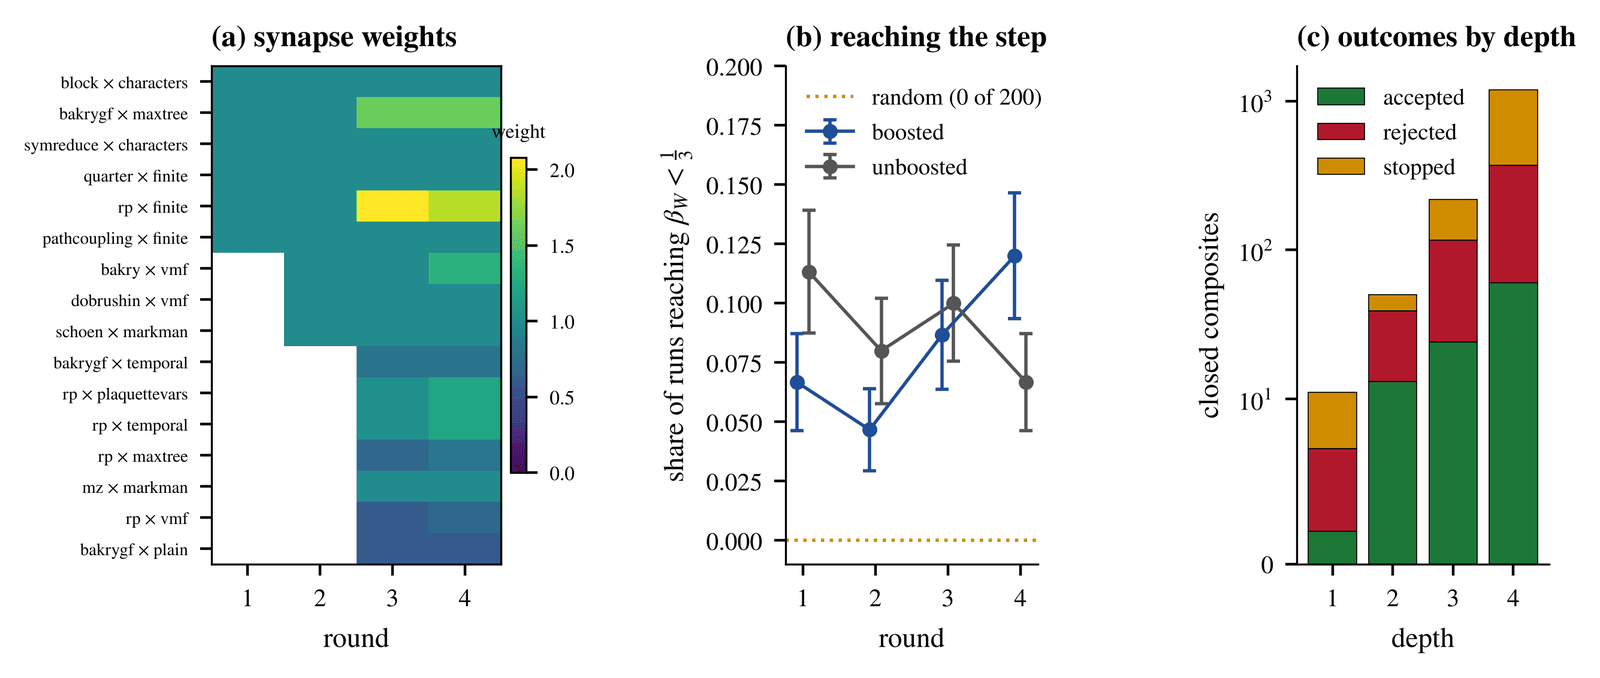
\includegraphics[width=0.98\textwidth]{figures/fig_boosters}
\caption{The booster layer. (a) The weights of the synapses of one boosted run over four rounds, one row per synapse; a blank cell is a synapse not yet created. (b) The share of $200$ runs that reach $\beta_{W}<\frac13$ within $48$ crosses, for the boosted arm that keeps its weights from round to round and for the unboosted network, with one standard error; random pairing never reaches it. (c) The outcomes of the $1{,}466$ closed composites of the amplified library, by depth.}
\label{fig:boosters}
\end{figure*}

\begin{table}[t]
\caption{Boosted, unboosted and random crossing at a budget of $48$ crosses, $200$ runs per arm. ``Reached $\frac13$'' counts runs whose survivors include $\beta_{W}<\frac13$, with the mean generation at which they reach it; survivors and refuted offspring are means per run.}
\label{tab:boosters}
\centering
\footnotesize
\setlength{\tabcolsep}{3.5pt}
\begin{tabular}{@{}llrrrr@{}}
\toprule
Synapse & Arm & Reached $\frac13$ & Generation & Survivors & Refuted \\
\midrule
pair & boosted & $14$ & $5.86$ & $0.61$ & $1.14$ \\
head & boosted & $12$ & $5.58$ & $0.62$ & $1.16$ \\
-- & unboosted & $21$ & $5.43$ & $0.68$ & $1.25$ \\
-- & random & $0$ & -- & $0.08$ & $0.05$ \\
\bottomrule
\end{tabular}
\end{table}

Boosters do not beat the unboosted network (Table~\ref{tab:boosters}). Within one round the boosted arms reach the step in $12$ and $14$ of $200$ runs against $21$ for the unboosted network; the difference is within two standard errors. Across four rounds the boosted share moves from $0.067$ to $0.12$ and the unboosted share from $0.113$ to $0.067$, again within two standard errors in every round. Both are far above random pairing, which wastes $45$ of its $48$ crosses on ill-typed pairs and never reaches the step. The reason is the one met in Section~\ref{ssec:crossing}: a booster strengthens synapses that have already fired, and the step that moved needed a synapse that had never fired, between Dobrushin's criterion and the maximal-tree gauge. The typing, not the learning, carries the advantage of the network.

\subsection{Gap numbers and the construction graph}\label{ssec:gapnumbers}

\emph{Gap numbers.} Each round reports two numbers. For Yang--Mills it is the largest coupling below which the lattice gap is proved, and its share of the interval up to $\beta_{W}\approx2.2$, where Monte Carlo simulations of four-dimensional $\mathrm{SU}(2)$ see the crossover from strong to weak coupling \cite{Cre80}; this is a physical marker and not the threshold of any proof, since Ba{\l}aban's control is not explicit in the coupling. The number moved from $\frac29$, or $10.1\%$, before the rounds to $\frac13$, or $15.2\%$, in the first round, and stayed there in the second. For Hodge it is, for each open family, the largest dimension of a family on whose general member the classes are known to be algebraic, against the dimension of the largest family of its kind (Table~\ref{tab:closure}). No Hodge number moved.

\begin{table*}[t]
\caption{The leaves of the two benchmark trees after the second round, with the result that settles a proved leaf, the check that stopped the last attempt on an open one, and, for the open families of the Hodge tree, the gap number: the largest dimension of a family on whose general member the classes are known to be algebraic, against the dimension of the largest family of its kind. Yang--Mills: $3$ of $8$ leaves proved ($37.5\%$); Hodge: $2$ of $10$ ($20\%$).}
\label{tab:closure}
\centering
\footnotesize
\setlength{\tabcolsep}{4pt}
\begin{tabular}{@{}rp{0.22\textwidth}p{0.08\textwidth}p{0.55\textwidth}p{0.07\textwidth}@{}}
\toprule
& Leaf & Status & Source, or what blocks & Gap \\
\midrule
\multicolumn{5}{@{}l}{\emph{Yang--Mills}}\\
\rr 1 & \rr a faithful Lean statement of the Clay problem & \rr blocked & \rr no formal statement of the Wightman axioms for a gauge theory exists to state it against & \rr -- \\
\rr 2 & \rr lattice gap at strong coupling & \rr proved & \rr $\beta_{W}<\frac29$ \cite{BB26d} & \rr -- \\
\rr 3 & \rr fine-scale control at weak coupling & \rr proved & \rr Ba{\l}aban's renormalisation group \cite{Bal87} & \rr -- \\
\rr 4 & \rr the window from below & \rr proved & \rr $\beta_{W}<\frac13$, Theorem~\ref{thm:onethird}; the ceiling of the method, Proposition~\ref{prop:forestceiling} & \rr $15.2\%$ \\
\rr 5 & \rr a finite-box mixing certificate in the window & \rr open & \rr the box needs side about $90$; no computation over $\mathrm{SU}(2)^{4n^{4}}$ at that size exists & \rr -- \\
\rr 6 & \rr a lift of the two-dimensional gap through dimension & \rr open & \rr no family of theories interpolating in dimension with a uniform gap is known & \rr -- \\
\rr 7 & \rr a multiscale log-Sobolev inequality at order-one coupling & \rr open & \rr the method of \cite{BB21} needs a Polchinski flow with uniformly convex effective potentials; for gauge fields none is known, and gauge invariance removes the Gaussian reference measure & \rr -- \\
\rr 8 & \rr the continuum limit with the Wightman axioms & \rr open & \rr needs a lattice gap uniform in the spacing, Hypothesis~R, which is the Clay problem on the lattice & \rr -- \\
\midrule
\multicolumn{5}{@{}l}{\emph{Hodge}}\\
\rr 1 & \rr a faithful Lean statement & \rr blocked & \rr Hodge classes and algebraic cycles of complex projective varieties are not yet formalised & \rr -- \\
\rr 2 & \rr (F2) in dimension at most five & \rr proved & \rr \cite{Mar25w,MZ98} & \rr -- \\
\rr 3 & \rr (F2) for CM abelian varieties & \rr open & \rr the only claim is unrefereed \cite{OAI26b}; the refuter rejects it & \rr -- \\
\rr 4 & \rr Weil classes on Weil eightfolds of nontrivial discriminant & \rr open & \rr no construction of the classes is known & \rr $0/16$ \\
\rr 5 & \rr a semiregular object on $E_{0}^{6}$ meeting the polarised criterion & \rr open & \rr every convolution tested in \cite{BB26c} has too large an $\mathrm{Ext}^{2}$ & \rr -- \\
\rr 6 & \rr Weil classes on Weil sixfolds & \rr open & \rr products of Weil fourfolds and Weil surfaces fill a family of dimension $5$ in the moduli of dimension $9$; a very general Weil sixfold is simple & \rr $5/9$ \\
\rr 7 & \rr (F3$'$) for $S\times S$, $S$ a K3 surface with real multiplication & \rr open & \rr $\sqrt d$ is a Hodge similitude; Varesco's reduction to the Kuga--Satake Hodge conjecture \cite{Var23} covers the first four-dimensional families, the largest family has dimension $8$ & \rr $4/8$ \\
\rr 8 & \rr Fermat fourfolds, degrees with split characters & \rr proved & \rr Shioda's zero-sum criterion \cite{Shi79} with the census of \cite{BB26c} & \rr -- \\
\rr 9 & \rr the Fermat fourfold of degree $110$ & \rr open & \rr the leftover character has a lattice point in its Fine interior, so no block family covers it, and its orbit under the symmetries has no split member & \rr one orbit \\
\rr 10 & \rr the Fermat fourfold of degree $220$ & \rr open & \rr the classes lifted from degree $110$ & \rr -- \\
\bottomrule
\end{tabular}
\end{table*}

\emph{What blocks.} On Yang--Mills the step that blocks is Hypothesis~R: a lattice gap uniform in the spacing, for which Ba{\l}aban's effective action at a fixed physical scale must land in a region where a convergent method applies. The strong-coupling side now reaches $\beta_{W}=\frac13$, the ceiling of single-link arguments after any forest gauge fixing, and going further needs multi-link blocks whose joint laws are controlled at finite coupling. On Hodge every open leaf is blocked by the absence of a construction of the classes: of Weil classes off the products of lower Weil varieties, of the classes of $\sqrt d$ on squares of K3 surfaces outside Varesco's families, and of the leftover class of the Fermat fourfold of degree $110$.

\emph{The construction graph.} The package records every node, every crossing with its parents, check and refuter verdict, the synapse weights of every run, and the map of the other workstreams that feed the library (Fig.~\ref{fig:graph}). Four workstreams feed it. The Yang--Mills archive \cite{BB26d} gives the sharp quarter, reflection positivity and the box criterion; the Hodge papers \cite{BB26c} give the split into (F2) and (F3$'$) and the open families; the census of Fermat varieties gives the characters left at $110$ and $220$; and the weighted-poset lemma of Section~\ref{ssec:crossing} gives the pattern of a change of representation, which the amplified round transfers to plaquette variables, blocks and the quotient of Fermat characters. The work on the lattice $D_{4}$ and the $24$-cell gives the pattern of a finite certificate, which the box nodes use. The Lehmer and Earth--Moon workstreams feed neither tree.

\begin{figure*}[t]
\centering
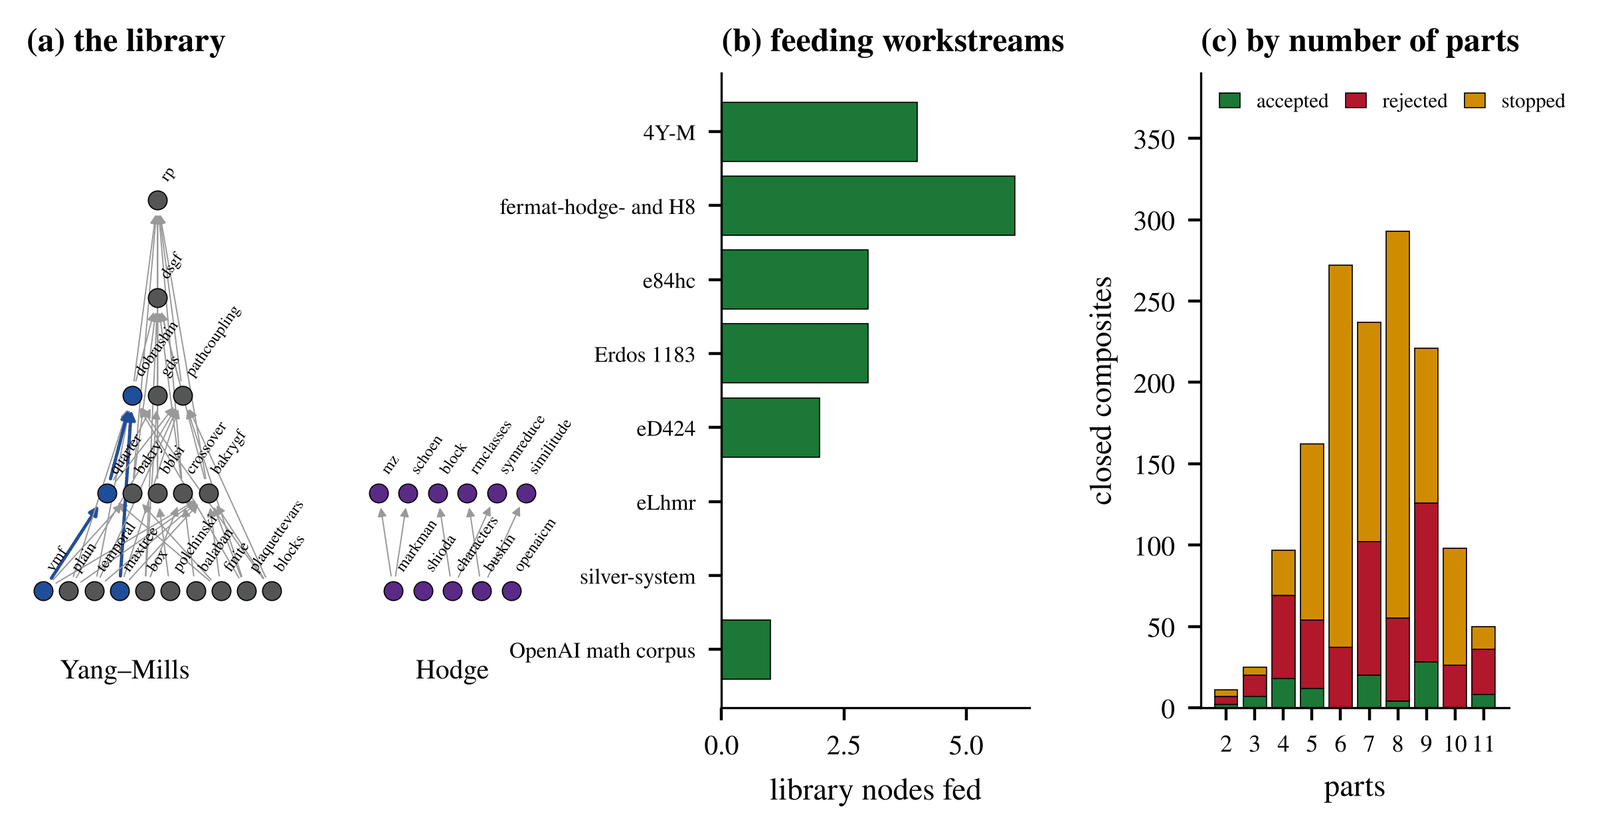
\includegraphics[width=0.98\textwidth]{figures/fig_graph}
\caption{The construction graph. (a) The library of the amplified round, with an arrow from $b$ to $a$ when $b$ can be fed into $a$, layered by the length of the longest chain of inputs; Yang--Mills nodes on the left, Hodge nodes on the right, and the four parents of the composite that proves $\beta_{W}<\frac13$ in blue. (b) The number of library nodes fed by each workstream. (c) Closed composites of the amplified library by number of parts and outcome.}
\label{fig:graph}
\end{figure*}
